\section{Back end}
\subsection{Descrizione generale}
\subsubsection{Comunicazione tra client e server}
Per la creazione del back end di MaaS si è deciso di utilizzare Node.js e, in particolare, il framework ExpressJS, che permette la creazione semplificata di server REST. Il lato back end sarà quindi costituito da un insieme di API protette da strati diversi di sicurezza. \\
Ciascuna API del webserver fornirà una risposta in formato JSON per permettere la fruizione delle informazioni. Fornirà nello stesso formato anche gli eventuali messaggi di errore generati nel corpo dei metodi del server. Tali messaggi di errore saranno così composti: 
\begin{verbatim}
{
    "code":     [Codice definito nel protocollo HTTP, che identifica univocamente
                 la tipologia del problema]
    "message":  [Messaggio che definisce in dettaglio la tipologia dell'errore]
    ["data":   [Opzionale, trasporta i dati in cui si è verificato l'errore]]
}
\end{verbatim}
I codici di errore saranno del tipo 4xx (client error, la richiesta è sintatticamente scorretta o non può essere soddisfatta) o 5xx (server error, il server ha fallito nel soddisfare una richiesta apparentemente valida).
\subsubsection{Sicurezza}
Gli accessi alle API avranno 2 livelli di sicurezza. \\
Il primo livello è rappresentato dall'autenticazione: un utente non autenticato riceverà un errore se richiede una API protetta. Verrà implementato con l'utilizzo di PassportJS, un middleware per ExpressJS che permette l'autenticazione di utenti nel sistema. In particolare verrà utilizzata la strategia passport-local per l'accesso al server, cioè le credenziali dell'utente risiederanno nel database locale. \\
Il secondo livello è definito in base al ruolo di appartenenza di un utente. Si occuperà di controllare i permessi assegnati ad un utente autenticato e di verificare la possibilità che possa o meno interagire con la risorsa richiesta. \\
I ruoli utente ammessi nell'applicazione sono: 
\begin{itemize}
\item \textbf{GUEST};
\item \textbf{MEMBER};
\item \textbf{ADMIN};
\item \textbf{OWNER};
\item \textbf{SUPERADMIN}.
\end{itemize}
Per il ruolo di SUPERADMIN è abilititato un set di API per la gestione dell'intera applicazione. Tali API non sono accessibili agli utenti con altri ruoli.
\subsection{Package e classi}
Nei seguenti due diagrammi vengono mostrate le relazioni generali tra i package e le relazioni tra le classi al loro interno. Successivamente, per ogni package verranno descritte le classi che li compongono.
\begin{figure}[h]
\centering
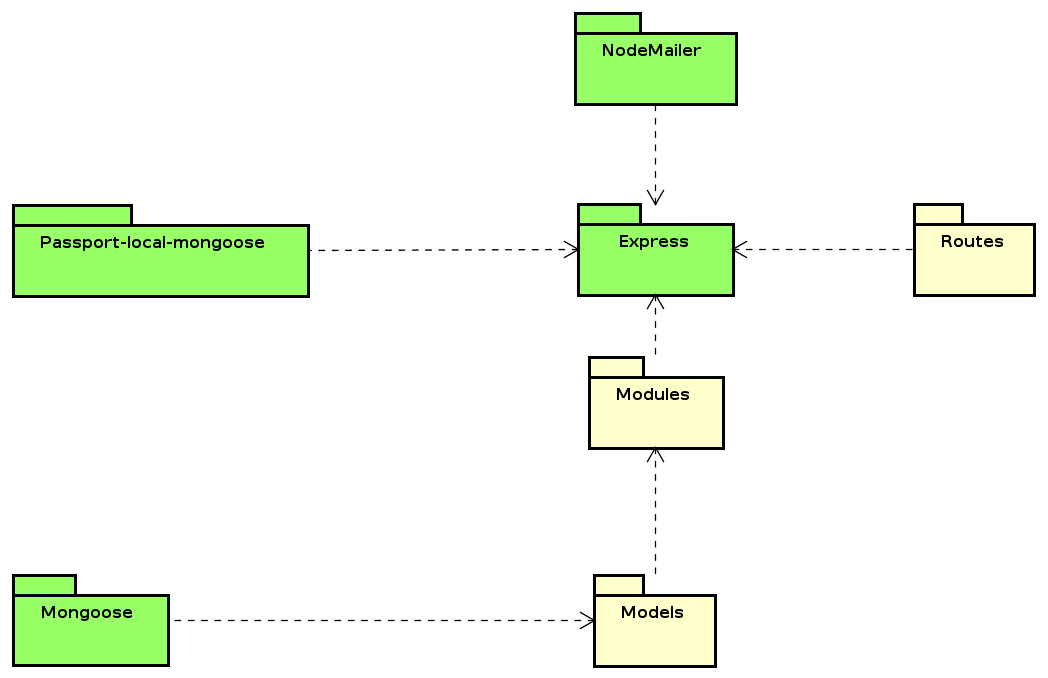
\includegraphics[width=0.8\textwidth]{res/sections/backend/package.png}
\caption{Diagramma generale dei package per il backend}
\end{figure}
\newpage
\begin{figure}[h]
\centering
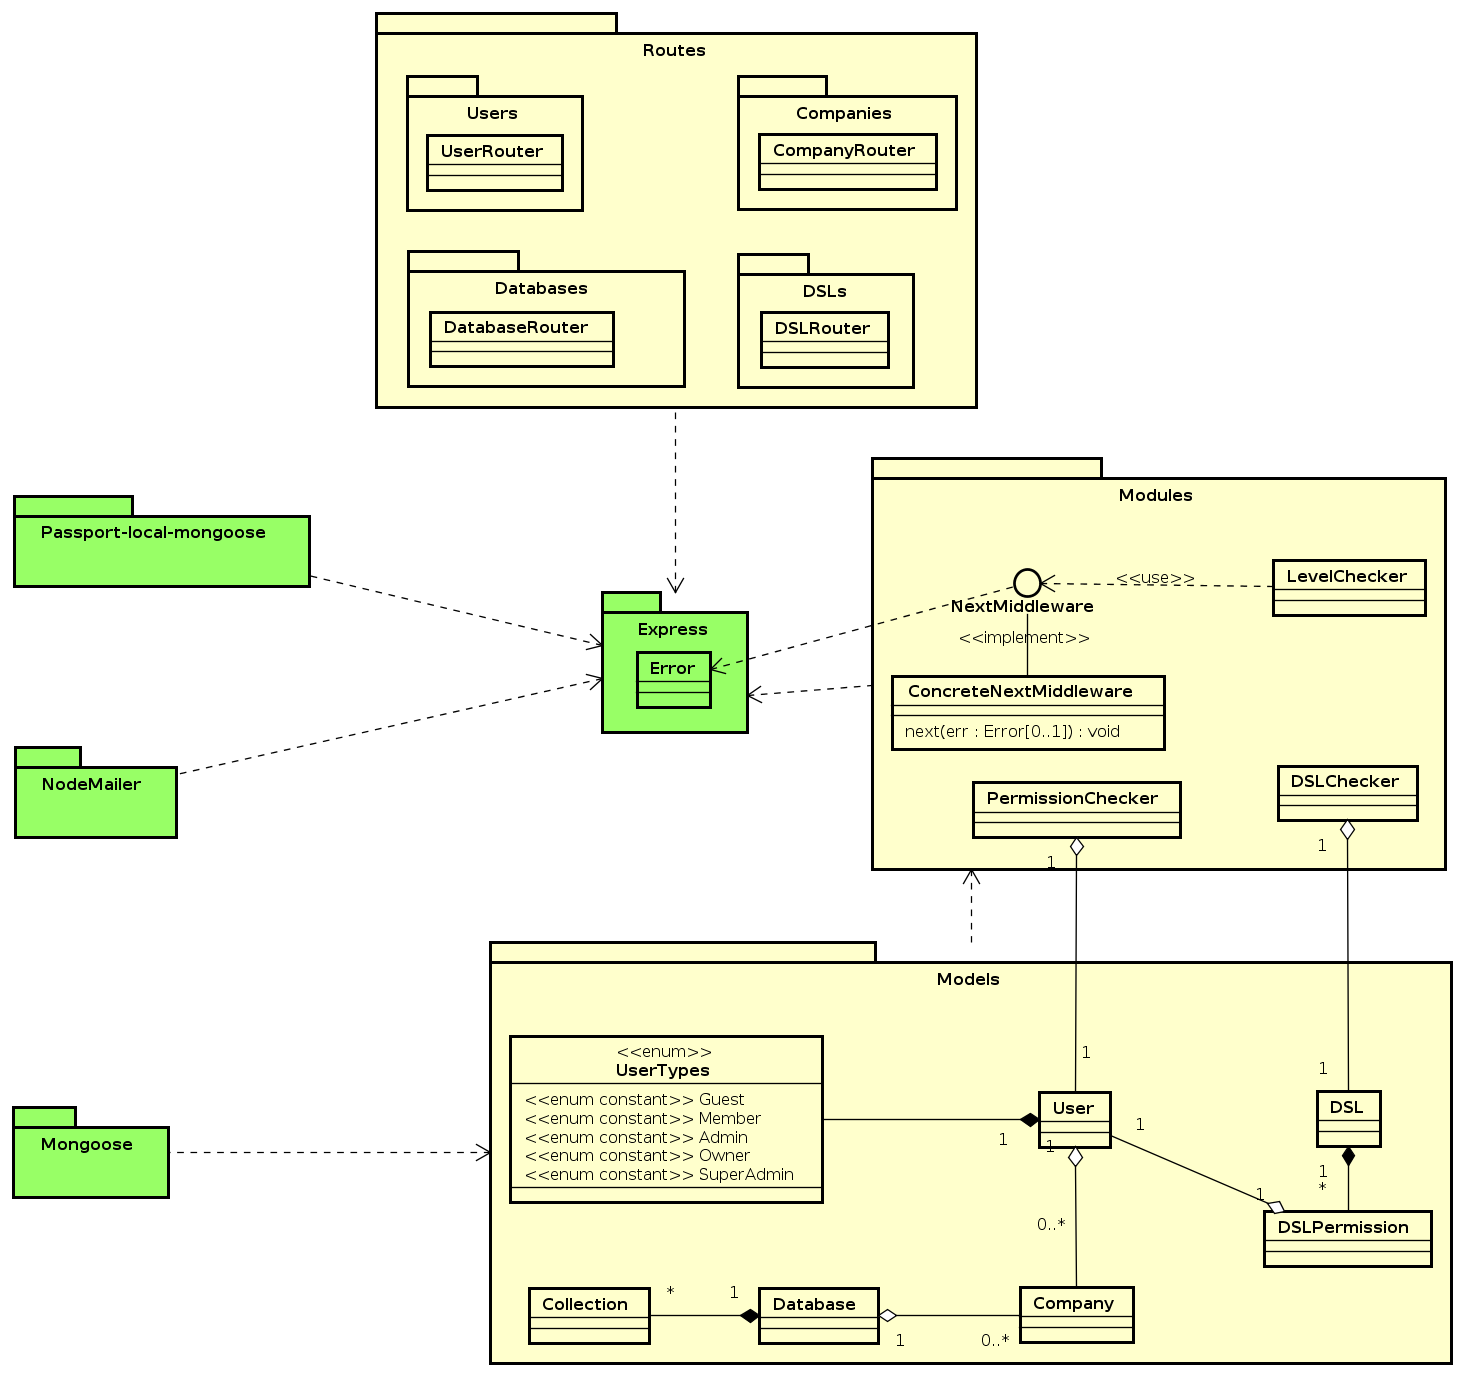
\includegraphics[width=0.8\textwidth]{res/sections/backend/packageWithClasses.png}
\caption{Diagramma generale dei package per il backend, comprensivo delle classi}
\end{figure}
\subsubsection{Models}
\begin{figure}[h]
\centering
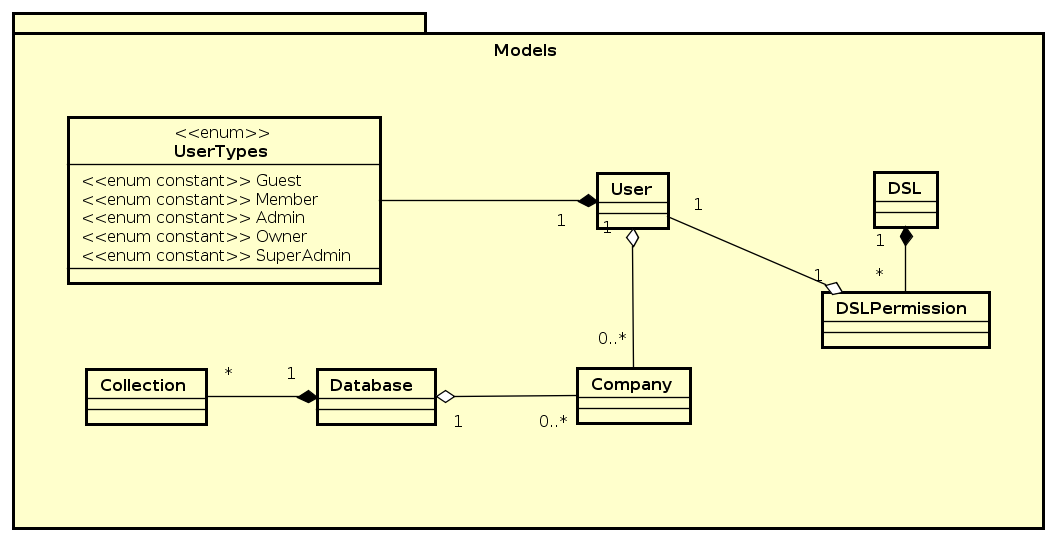
\includegraphics[width=0.8\textwidth]{res/sections/backend/Models.png}
\caption{Diagramma delle classi per il package Models}
\end{figure}
\paragraph{Descrizione} \mbox{}\\
In questo package sono definiti i modelli di dato che rappresentano il core business dell'applicazione:
\begin{itemize}
\item User;
\item Company;
\item DSL;
\item Database.
\end{itemize}
Questi quattro modelli sono rappresentati da altrettante classi, che si occupano di interagire con il database MongoDB dell'applicazione, attraverso Mongoose, al fine di effettuare operazioni CRUD sui dati. Per restringere l'accesso ad alcune collection del database e/o alle specifiche DSL, vegono fornite altre due classi, che si occuano di memorizzare i permessi associati alle collections (in base al ruolo dell'utente) e alle specifiche DSL (in base all'utente stesso). Questo package rappresenta la parte M (Model) del design pattern MVC.
\paragraph{Classi contenute}
\begin{itemize}
\item User;
\item Company;
\item DSL;
\item Database;
\item Collection;
\item DSLPermission.
\end{itemize}
\subparagraph{User}
\begin{description}
\item[Descrizione] \hfill \\
Questa classe si occupa di fornire metodi di utilità per gestire i dati di un utente dell'applicazione. Per ogni utente viene inoltre memorizzata Company di appartenenza: l'owner (o gli owner) verranno riconosciuti perché il loro tipo, individuato dall'enum UserTypes, sarà corrispondente a Owner.
\item[Utilizzo] \hfill \\
Viene utilizzata per l’interfacciamento con la libreria Mongoose per la registrazione dello schema dei dati degli utenti, e con la libreria passport-local-mongoose per il popolamento automatico dello schema con campi dati e metodi predefiniti. Fornisce metodi per la modifica, e visualizzazione, del profilo e di modifica delle credenziali di accesso, oltre che metodi di creazione e cancellazione di un utente.
\end{description}
\subparagraph{Company}
\begin{description}
\item[Descrizione] \hfill \\
Questa classe si occupa di fornire metodi di utilità per gestire i dati di una company.
\item[Utilizzo] \hfill \\
Viene utilizzata per l’interfacciamento con la libreria Mongoose per la registrazione dello schema dei dati delle companies. Fornisce metodi per la modifica dei dati della company, oltre che per l'aggiunta/rimozione della stessa.
\end{description}
\subparagraph{DSL}
\begin{description}
\item[Descrizione] \hfill \\
Questa classe si occupa di fornire metodi di utilità per gestire i dati di una specifica DSL.
\item[Utilizzo] \hfill \\
Viene utilizzata per l’interfacciamento con la libreria Mongoose per la registrazione dello schema dei dati delle specifiche DSL. Offre metodi per aggiungere, modificare, visualizzare ed eseguire specifiche DSL. Al fine di garantire consistenza con i permessi, viene fornita anche una classe DSLPermission, che rappresenta un generico permesso sulla specifica DSL fornito ad un utente.
\end{description}
\subparagraph{Database}
\begin{description}
\item[Descrizione] \hfill \\
Questa classe si occupa di fornire metodi di utilità per gestire i dati dei database registrati da una company.
\item[Utilizzo] \hfill \\
Viene utilizzata per l’interfacciamento con la libreria Mongoose per la registrazione dello schema dei dati dei database. Fornisce metodi per la modifica dei dati di un database (consentendo l'aggiunta di collection e restrizioni su di esse), oltre che per l'aggiunta/rimozione. Al fine di poter impostare restrizioni sull'accesso ad alcune collection da parte degli utenti member, viene fornita anche una classe Collection, che definisce se la corripondente collection del database è accessibile o no da un utente che non sia almeno admin.
\end{description}
\subparagraph{Collection}
\begin{description}
\item[Descrizione] \hfill \\
Questa classe si occupa di definire permessi sulle collections di un database della company, per impedire che un member possa accedervi.
\item[Utilizzo] \hfill \\
Viene utilizzata per memorizzare permessi definiti a livello di ruolo sulle collections di un database di una company. Alcune collections potrebbero non dover essere accedute da semplici member: questa classe memorizza il nome della collection e se può essere acceduta da member o meno.
\end{description}
\subparagraph{DSLPermission}
\begin{description}
\item[Descrizione] \hfill \\
Questa classe si occupa di definire permessi sulle specifiche DSL.
\item[Utilizzo] \hfill \\
Viene utilizzata per memorizzare permessi definiti a livello di utente sulle specifiche DSL. Alla creazione di una specifica DSL, l'utente che l'ha creata viene registrato come proprietario. I permessi definiti da questa classe sono scrittura ed esecuzione, in quanto si assume che nessuno possa leggere il codice della specifica DSL senza poterlo modificare. Se un utente non ha definito un permesso DSLPermission per una specifica DSL significa che quell'utente non gode di nessun permesso.
\end{description}
\subsubsection{Modules}
\begin{figure}[h]
\centering
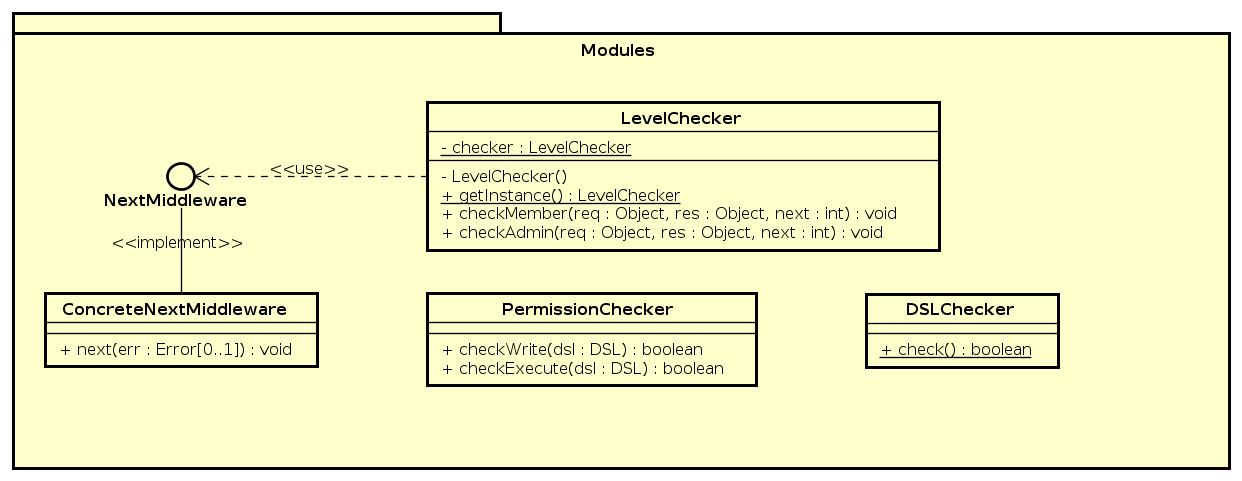
\includegraphics[width=0.8\textwidth]{res/sections/backend/Modules.png}
\caption{Diagramma delle classi per il package Modules}
\end{figure}
\paragraph{Descrizione} \mbox{}\\
In questo package sono contenute tutte le utility utilizzate dall'applicazione per controllare se il ruolo dell'utente è sufficiente a fargli eseguire l'operazione richiesta, se la specifica DSL inviata è sintatticamente corretta e se l'utente ha il permesso di eseguire l'operazione di scrittura/esecuzione sulla specifica DSL invocata.
\paragraph{Classi contenute}
\begin{itemize}
\item PermissionChecker;
\item LevelChecker;
\item DSLChecker;
\end{itemize}
\subparagraph{PermissionChecker}
\begin{description}
\item[Descrizione] \hfill \\
Questa classe si occupa di controllare che un utente abbia il permesso di eseguire un'operazione (di lettura o esecuzione, come specificato nella descrizione della classe DSLPermission) su una specifica DSL.
\item[Utilizzo] \hfill \\
Viene utilizzata per capire se consentire o meno l'accesso in esecuzione o scrittura ad una specifica DSL.
\end{description}
\subparagraph{LevelChecker}
\begin{description}
\item[Descrizione] \hfill \\
Questa classe si occupa di controllare che un utente abbia il ruolo necessario ad eseguire l'operazione invocata. Molte operazioni, infatti, richiedono un ruolo minimo per essere eseguite.
\item[Utilizzo] \hfill \\
Viene utilizzata per capire se consentire o meno l'esecuzione di un'operazione in base al ruolo dell'uente che l'ha invocata.
\end{description}
\subparagraph{DSLChecker}
\begin{description}
\item[Descrizione] \hfill \\
%todo
\item[Utilizzo] \hfill \\
%todo
\end{description}

\subsubsection{Routes}
\begin{figure}[h]
\centering
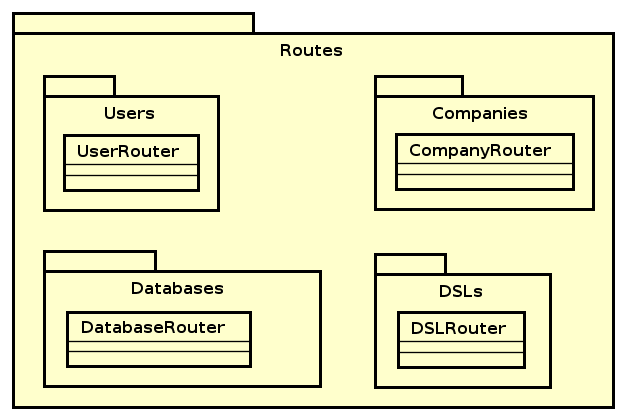
\includegraphics[width=0.8\textwidth]{res/sections/backend/Routes.png}
\caption{Diagramma delle classi per il package Routes}
\end{figure}
\paragraph{Descrizione} \mbox{}\\
In questo package sono presenti tutti i moduli contenenti le varie Routes. In ExpressJS, il routing ha il compito di determinare come l'applicazione risponde ad una richiesta del client verso un particolare endpoint. L'endpoint è semplicemente una coppia formata da un URI e da un metodo di richiesta (GET, POST, PUT o DELETE). Ogni route può avere una o più funzioni associate che bengono eseguite quando la route è invocata. Le Routes rappresentano la parte C (Controller) del design pattern MVC.
\paragraph{Package contenuti}
\begin{itemize}
\item Users;
\item DSLs;
\item Companies;
\item Databases.
\end{itemize}
\subparagraph{UserRouter} \mbox{}\\
In questo package è contenuto il router per le richieste che coinvolgono il modello di dati User. Questa classe si chiama UserRouter, ed ha il compito di determinare come l'applicazione risponde alle richieste del client che coinvolgono l'endpoint degli utenti. 
\subparagraph{DSLRouter} \mbox{}\\
In questo package è contenuto il router per le richieste che coinvolgono il modello di dati DSL. Questa classe si chiama DSLRouter, ed ha il compito di determinare come l'applicazione risponde alle richieste del client che coinvolgono l'endpoint delle specifiche DSL. 
\subparagraph{CompanyRouter} \mbox{}\\
In questo package è contenuto il router per le richieste che coinvolgono il modello di dati Company. Questa classe si chiama CompanyRouter, ed ha il compito di determinare come l'applicazione risponde alle richieste del client che coinvolgono l'endpoint delle company. 
\subparagraph{DatabaseRouter} \mbox{}\\
In questo package è contenuto il router per le richieste che coinvolgono il modello di dati Database. Questa classe si chiama databaseRouter, ed ha il compito di determinare come l'applicazione risponde alle richieste del client che coinvolgono l'endpoint dei database. 